\chapter[Metodologia]{Metodologia}\label{chap:metodologia}
Este Capítulo aborda a metodologia usada no desenvolvimento desse trabalho. Organizado em seções, têm-se:
Seção de \hyperref[sec:classpesq]{Classificação de Pesquisa}, que apresenta a abordagem, a natureza, os objetivos
e os procedimentos desse trabalho; Seção de \hyperref[sec:metdev]{Metodologia do} \hyperref[sec:metdev]{Desenvolvimento}, a qual traz 
a metodologia usada para auxiliar durante o desenvolvimento; Seção 
\hyperref[sec:expus]{Metodologia de Coleta e Análise dos Resultados}, detalha o processo de coleta e análise
dos resultados obtidos; Seção \hyperref[sec:fluxoatv]{Fluxo das atividades}, que apresenta o fluxograma das atividades desse 
trabalho, bem como um detalhamento de cada etapa; Seção \hyperref[sec:cronog]{Cronogramas}, que mostra o cronograma definido 
para esse trabalho. Por fim, na Seção 
\hyperref[sec:resmet]{Resumo do Capítulo} são apresentadas as considerações finais
do capítulo.

\section{Classificação de Pesquisa}\label{sec:classpesq}

De acordo com \mycitetext{gil2010elaborar}, pesquisa é um procedimento racional e sistemático que visa trazer soluções à problemas propostos.
E ainda, que a pesquisa se desenvolve mediante o uso do conhecimento disponível, da utilização de técnicas e outros 
procedimentos científicos. Nesse contexto, a metodologia entra como um validador do caminho escolhido para conduzir a pesquisa,
vai além das descrições técnicas dos métodos, cuja função é guiar e estabelecer regras e procedimentos para a realização
da pesquisa \cite{gerhardt2009metodos}.
A pesquisa, se classifica quanto sua abordagem, natureza, objetivos e procedimentos. Nesta Seção, será abordado em quais 
classficações esse trabalho está inserido, contextualizando sua relevância e aplicação desses conceitos na
prática de pesquisa acadêmica e científica.

\subsection{Abordagem}\label{subsec:abord}

A Abordagem será híbrida, trazendo aspectos da abordagem qualitativa ao avaliar a satisfação do usuário ao utilizar o sistema,
de maneira subjetiva, levando em conta a particularidade de cada usuário, principalmente ao considerar que Sistemas de Recomendação
são voltados unicamente para os usuários e a experiência de cada um pode variar de acordo com seu perfil. Mas também apresentará
aspectos da abordagem quantitativa ao utilizar de métricas de precisão e acurácia de modelos de Inteligência Artificial, 
trazendo dados númericos resultantes de uma avaliação estatística do modelo.

\subsection{Natureza}\label{subsec:nat}

A Natureza da pesquisa é aplicada, pois é voltada para a solução de um problema específico de como se pode desenvolver um Sistema
de Recomendação com IA e como esse sistema proporciona maior satisfação aos seus usuários. 

\subsection{Objetivos}\label{subsec:obj}

Esse trabalho será caracterizado como pesquisa exploratória, já que esse tipo de pesquisa facilitam a familiariedade do pesquisador com o objeto de 
pesquisa, para assim tornar a questão mais clara, no caso, o uso de Inteligência Artificial em Sistemas de Recomendação e como
esse uso pode trazer satisfação aos seus usários. 

\subsection{Procedimentos}\label{subsec:proced}

Quanto aos procedimentos, esse trabalho utiliza de pesquisa bibliográfica, sendo esta um tabalho exploratório que busca
aumentar o conhecimento do autor sobre o assunto abordado, é a base teórica do estudo \cite{nascimento2016classificaccao}.
Além desse, esse trabalho ainda utiliza de pesquisa-ação, onde certa situação-problema é investigada, o uso de Inteligência Artificial
em Sistemas de Recomendação, e em discussão com pessoas, no caso os usuários, procura-se chegar à uma resolução e gerar aprendizado
sobre a situação. Nesse contexto, este trabalho visa apresentar uma solução de Sistemas de Recomendação, validar com os usuários
sua satisfação, aprimorar a solução e novamente validar com os usuários a eficiência da solução.

\section{Metodologia do Desenvolvimento}\label{sec:metdev}

Essa seção apresenta a metodologia utilizada durante o desenvolvimento da aplicação proposta. Para este trabalho, será utilizado
elementos da metodologia ágil Scrum que mais se encaixam com o contexto do que será desenvolvido.

O Scrum é uma metodologia que atua como um guia, com papéis bem definidos e que traz visibiliadade ao autor do projeto sobre 
exatemente como está seu andamento \cite{pereira2007entendendo}. Este possui um conjunto papéis, eventos, artefatos e regras
que auxiliam os usuários de Scrum a se orientarem durante o projeto. Ao trazer o Scrum para este trabalho, levando em conta principalmente
sua versatilidade e a agilidade que ele permite que seja o acompanhamento do projeto, será utilizado eventos como sprints, 
reuniões de planejamento e o \textit{Sprint Burndown}, que mapeia o progresso da sprint em forma de gráfico. Foram separado esses
eventos do Scrum, ao considerar que a autora desenvolverá sozinha o trabalho. Sendo assim, algumas outras atividades do Scrum, como
\textit{Dailys} ou Retrospectivas que são mais voltadas para um time, perdem o sentido de serem realizadas. Mas ainda sim, será
acompanhado o progresso por sprint através do \textit{Sprint Burndown}.

\begin{itemize}
    \item Sprint: As sprints são uma série iterações com um tempo definido, no caso desse trabalho, sprints de duas semanas, nas 
    quais são realizadas atividades que devem ser planejadas, feitas e entregues dentro do ciclo. Atividades as quais, incrementam
    o produto final de alguma forma. Assim, a cada iteração é gerado um novo produto de valor;   
    \item Reuniões de Planejamento: As reuniões de planejamento tem como objetivo definir quais e como as atividades serão realizadas
    na sprint. Para isso será definido um backlog para a parte de desenvolvimento, e será mapeado quais atividades serão realizadas
    durante cada sprint, e
    \item \textit{Sprint Burndown}: São gráficos que mostram o andamento das atividades de cada sprint. Será utilizado mais como
    métrica de acompanhamento, para verificar o andamento do trabalho e se as sprints estão sendo finalizadas como esperado.
\end{itemize}

Para o TCC 1, o backlog está definido pela Figura \hyperref[fig:backlogtcc1]{9}, já mapeado por sprints. Para o TCC 2, o backlog
deverá ser definido com base no cronograma e atividades a serem desenvolvidas durante a execução da segunda etapa do trabalho.

\begin{figure}[htbp]
    \centering
    \caption{Backlog - TCC 1}
    \label{fig:backlogtcc1}
    
    \vspace{2pt} % Espaço vertical entre a legenda e a imagem
    
    \includegraphics[width=1.0\textwidth]{figuras/backlogtcc1.eps}
    
    \vspace{2pt} % Espaço vertical entre a imagem e a fonte da imagem
    
    \small Fonte: Autora
\end{figure}

\section{Metodologia de Coleta e Análise dos Resultados}\label{sec:meteanresul}

Como abordado na Seção de \hyperref[sec:expus]{Satisfação do Usuário}, para a coleta de dados de satisfação do usuário 
será utilizado o modelo de \mycitetext{mahmood2000variables}, com o foco em benefícios e conveniência, antecedentes do usuário
e suporte e estímulo organizacional. Para elaboração do questionário, terá prioriadade de questões em escalas (0 a 10), para
que seja possível mensurar e aplicar os resultados no modelo, e uma questão subjetiva de opinião geral da aplicação pela
visão do usuário.

As perguntas serão desenvolvidas com base na base de dados escolhida, pois seus resultados devem ser usados para treinar novamente
o modelo e gerar uma versão mais precisa. O mesmo questionário será aplicado após o modelo re-treinado ser aplicado no sistema, assim
será analisado atráves das respostas se houve uma melhora no Sistema de Recomendação.

Além da análise com base na satisfação do usuário, terão métricas objetivas para avaliar o desempenho dos modelos, sendo elas:
\begin{itemize}
    \item Precisão: é uma métrica que mede a proporção de itens recomendados que são relevantes para o usuário;
    \[
    \text{Precisão} = \frac{\text{Número de itens relevantes recomendados}}{\text{Número total de itens recomendados}}
    \]
    \item Revocação: é uma métrica que mede a proporção de itens relevantes que foram corretamente recomendados pelo sistema, e
    \[
    \text{Revocação} = \frac{\text{Número de itens relevantes recomendados}}{\text{Número total de itens relevantes}}
    \]
    \item \textit{F1-Score}: é uma métrica que combina precisão e revocação, fornecendo uma medida geral do desempenho do 
    sistema. É calculado como a média harmônica entre precisão e revocação.
    \[
    \text{\textit{F1-Score}} = \frac{2 \times \text{Precision} \times \text{Recall}}{\text{Precision} + \text{Recall}}
    \]
\end{itemize}

\section{Fluxo das atividades}\label{sec:fluxoatv}

Essa seção é dedicada a apresentar as atividades realizadas durante a execução desse trabalho. Dividia em duas subseções,
mostra as atividades desenvolvidas durante a execução da primeira etapa desse trabalho, TCC 1, cujo foco é em embasar a 
questão de pesquisa com referenciais bibliográficos e apresentar uma proposta. Já na segunda etapa, TCC 2, o foco é 
desenvolver a proposta apresentada na primeira fase e atingir os objetivos definidos na seção 
\hyperref[sec:objetivos]{Objetivos}.

\subsection{TCC 1}\label{subsec:tcc1}

A Figura \hyperref[fig:bpmnTcc1]{10} e a Figura \hyperref[fig:subproccesstcc1]{11} apresentam em formato de gráfico BPMN (\textit{Business Process Modeling Notation}) 
o fluxo de atividades previstas para o TCC 1:

\begin{itemize}
\item Definir Tema: aqui será definido o tema no qual o trabalho será realizado;
\item Levantar Bibliográfia: aqui será levantado todo a base teórica a qual sustenta esse trabalho;
\item Descrever Introdução: aqui será desenvolvido a introdução do trabalho, trazendo uma ideia geral do tema e objetivos 
desse trabalho;
\item Descrever Referencial Teórico: aqui será abordado com mais detalhes as bases teóricas que auxiliaram na construção
do trabalho;
\item Descrever Suporte Tecnológico: aqui será descrito todas as tecnologias que apoaiaram o desenvolvimento do trabalho;
\item Descrever Metodologia: aqui será apresentada a metodologia e cronograma desse trabalho;
\item Desenvolver Provas de Conceito: aqui será iniciado parte do desenvolvimento do trabalho. Com o objetivo de selecionar
o melhor filtro e modelo de \textit{Deep Learning} para ser usado no trabalho, será desenvolvido provas de conceito a fim de,
com dados práticos, apontar o modelo a ser usado no trabalho;
    \begin{itemize}
        \item Separar parcialmente uma base de dados: selecionar uma pequena parte da base de dados para testar os modelos;
        \item Criar modelo de Filtro Colaborativo: com a base selecionada aplicar o Filtros Colaborativos nela e treinar um modelo;
        \item Criar modelo de Filtro de Conteúdo: com a base selecionada aplicar o Filtros de Conteúdo nela e treinar um modelo;
        \item Criar modelo de Filtro Demográficos: com a base selecionada aplicar o Filtros Demográficos nela e treinar um modelo;
        \item Criar modelo de Filtros Baseados em Conhecimento e Utilidade: com a base selecionada aplicar
         o Filtros Baseados em Conhecimento e Utilidade nela e treinar um modelo;
        \item Criar modelo de Filtro Híbridos: com a base selecionada aplicar o Filtros Híbridos nela e treinar um modelo;
        \item Analisar resultados dos filtros: tendo todos os modelos criados, analisar os resultados de acúracia de todos e escolher 
        o que tiver maior acúracia;
        \item Aplicação de Redes Neurais Convolucionais nos filtros escolhidos: tendo o filtro escolhido implementar 
        Redes Neurais Convolucionais e treinar novamente o modelo;
        \item Aplicação de Redes Neurais Recorrentes nos filtros escolhidos: tendo o filtro escolhido implementar 
        Redes Neurais Recorrentes e treinar novamente o modelo;
        \item Aplicação de Máquina de Boltzmann Restrita nos filtros escolhidos: tendo o filtro escolhido implementar 
        Máquina de Boltzmann Restrita e treinar novamente o modelo;
        \item Aplicação de Autoencoder nos filtros escolhidos: tendo o filtro escolhido implementar 
        Autoencoder e treinar novamente o modelo, e
        \item Analisar resultado da abordagem: analisar os resultados da aplicação dos metódos de \textit{Deep Learning}
        no modelo e escolher o com maior acúracia.
    \end{itemize}
\item Descrever Proposta: aqui será descrito a proposta que esse trabalho traz para solucionar as 
\hyperref[sec:questaopesquisa]{Questões de Pesquisa e Desenvolvimento};
\item Descrever Conclusões iniciais: aqui será descrito as conclusões iniciais, com base nas provas de conceito desenvolvidas
e na pesquisa realizada, e
\item Apresentar Monografia: aqui será apresentado o trabalho para à banca.
\end{itemize}

\begin{figure}[H]
    \centering
    \caption{Fluxo de Atividades TCC 1}
    \label{fig:bpmnTcc1}
    
    \vspace{2pt} % Espaço vertical entre a legenda e a imagem
    
    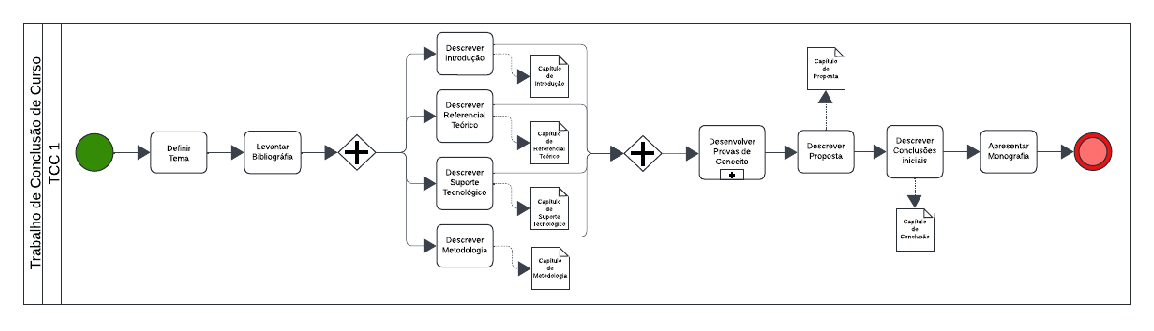
\includegraphics[width=1.0\textwidth]{figuras/bpmnTcc1.eps}
    
    \vspace{2pt} % Espaço vertical entre a imagem e a fonte da imagem
    
    \small Fonte: Autora
\end{figure}

\begin{figure}[H]
    \centering
    \caption{Subprocesso - Prova de Conceito - TCC 1}
    \label{fig:subproccesstcc1}
    
    \vspace{2pt} % Espaço vertical entre a legenda e a imagem
    
    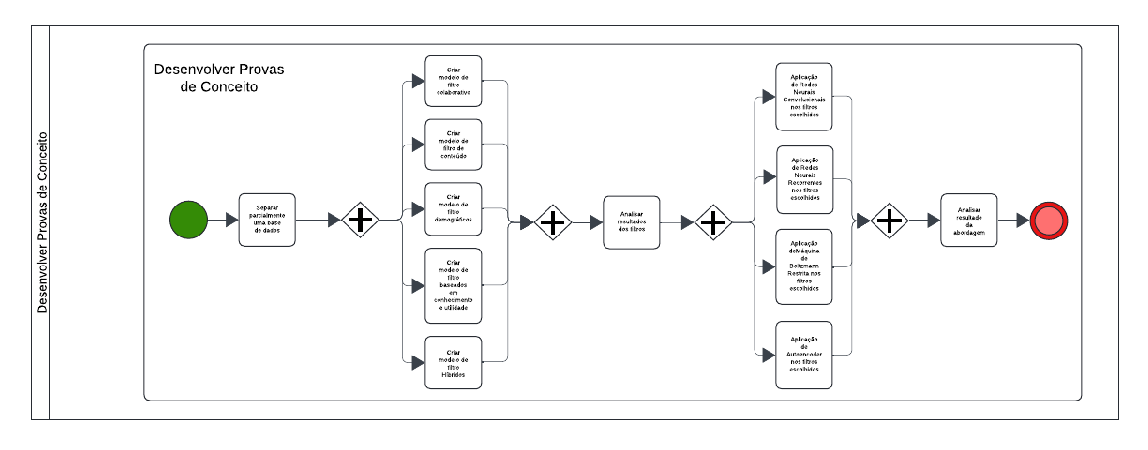
\includegraphics[width=1.0\textwidth]{figuras/subproccesstcc1.eps}
    
    \vspace{2pt} % Espaço vertical entre a imagem e a fonte da imagem
    
    \small Fonte: Autora
\end{figure}

\subsection{TCC 2}\label{subsec:tcc2}

A Figura \hyperref[fig:bpmnTcc2]{12} apresenta em formato de gráfico BPMN (\textit{Business Process Modeling Notation}) 
o fluxo de atividades previstas para o TCC 2:

\begin{enumerate}
    \item Aplicar correções da banca: aqui será aplicado ainda na primeira parte do trabalho as correções sugeridas pela banca;
    \item Separar base de dados: aqui será escolhido e manipulado qual será a base de dados a ser usada nesse trabalho;
    \item Desenvolver modelo de Sistema de Recomendação: aqui será desenvolvido o modelo de Sistema de Recomendação, com base
    nas Provas de Conceito realizadas na primeira parte do trabalho;
    \item Desenvolver API: aqui será desenvolvido a API que vai interagir com o usuário e apresentar o Sistema de Recomendação
    desenvolvido, com um foco maior no \textit{frontend} da aplicação;
    \item Aplicar modelo na API: aqui será aplicado o modelo de Sistema de Recomendação na aplicação desenvolvida;
    \item Analisar satisfação do usuário: aqui será capturado atráves de formulários a experiência do usuário com o Sistema de
    Recomendação desenvolvido;
    \item Aplicar satisfação do usuário para incrementar o modelo: aqui será separado os dados que podem ser aproveitados para
    incrementar o modelo e aplicá-los em um novo treinamento do modelo;
    \item Analisar novos resultados: aqui será novamente coletado a satisfação dos usuários e será analisado se o Sistema 
    de Recomendação ficou mais preciso;
    \item Refinar Monografia: aqui será revisado o trabalho e finalizado sua escrita, e
    \item Apresentar Monografia: aqui será a apresentação final do trabalho.
\end{enumerate}

\begin{figure}[H]
    \centering
    \caption{Fluxo de Atividades TCC 2}
    \label{fig:bpmnTcc2}
    
    \vspace{2pt} % Espaço vertical entre a legenda e a imagem
    
    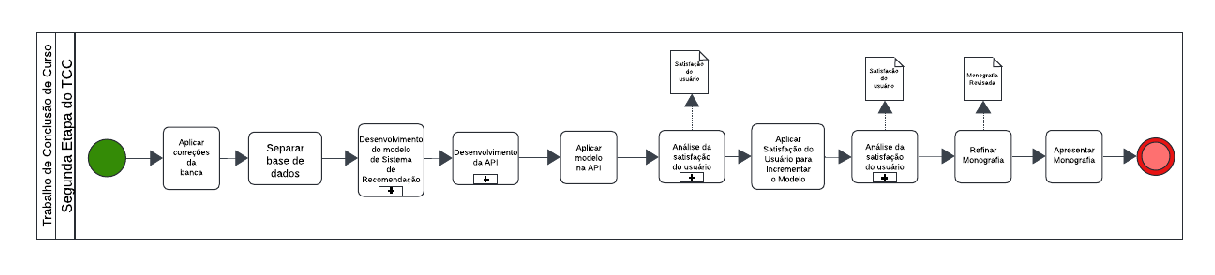
\includegraphics[width=1.0\textwidth]{figuras/bpmnTcc2.eps}
    
    \vspace{2pt} % Espaço vertical entre a imagem e a fonte da imagem
    
    \small Fonte: Autora
\end{figure}

\section{Cronogramas}\label{sec:cronog}

O Quadro \hyperref[tab:3]{3} apresenta os meses previstos para cada atividade do TCC 1.

\begin{table}[htbp]
    \centering
    \begin{threeparttable}
        \caption{Cronograma de atividades TCC1}
        \label{tab:3}
        \begin{tabular}{>{\raggedright\arraybackslash}m{6cm} c m{1cm} c c c}
        \toprule 
        Atividades & Março & Abril & Maio & Junho & Julho \\
        \midrule
        Definir Tema & X &  &  &  & \\
        \hline 
        Levantar Bibliográfia & X &  &  &  & \\
        \hline 
        Descrever Introdução & X &  &  &  & \\
        \hline 
        Descrever Referencial Teórico &  & X & &  & \\
        \hline 
        Descrever Suporte Tecnológico & & X & &  & \\
        \hline 
        Descrever Metodologia &  & X &  X &  & \\
        \hline 
        Desenvolver Prova de Conceito &  &  & X & X & \\
        \hline 
        Descrever Proposta &  &  & X & X & \\
        \hline 
        Descrever Conclusões iniciais &  &  &  & X & \\
        \hline
        Apresentar Monografia &  &  &  & & X \\
        \bottomrule 
        \end{tabular}
        \begin{tablenotes}
            \small
            \centering
            \item Fonte: Autora
        \end{tablenotes}
    \end{threeparttable}
\end{table}

O Quadro \hyperref[tab:4]{4} apresenta os meses previstos para cada atividade do TCC 2.

\begin{table}[htbp]
    \centering
    \begin{threeparttable}
        \caption{Cronograma de atividades TCC2}
        \label{tab:4}
        \begin{tabular}{>{\raggedright\arraybackslash}m{6cm} c m{1cm} c c c}
        \toprule 
        Atividades & Julho & Agosto & Setembro & Outubro & Novembro \\
        \midrule
        Aplicar Correções da Banca & X &  &  &  & \\
        \hline 
        Desenvolver Modelo de Sistema de Recomendação & X & X &  &  & \\
        \hline 
        Desenvolver API & X & X &  &  & \\
        \hline 
        Aplicar Modelo na API &  & X &  &  & \\
        \hline 
        Analisar Resultados &  & X & &  & \\
        \hline 
        Usar os resultados para incrementar o modelo &  & X & &  & \\
        \hline 
        Reaplicar novo modelo na API &  &  & X &  & \\
        \hline 
        Analisar novos resultados &  &  & X &  & \\
        \hline 
        Refinar Monografia &  &  &  & X & \\
        \hline
        Apresentar Monografia &  &  &  & & X \\
        \bottomrule 
        \end{tabular}
        \begin{tablenotes}
            \small
            \centering
            \item Fonte: Autora
        \end{tablenotes}
    \end{threeparttable}
\end{table}

\section{Resumo do Capítulo}\label{sec:resmet}
Neste capítulo foi apresentado a Classificação de Pesquisa, quanto à Natureza, aplicada; Abordagem, híbrida; Objetivos, 
exploratório, e Procedimentos, pesquisa Bibliográfia/ Pesquisa-ação. Também foi abordado a Metodologia do 
Desenvolvimento, que será Scrum e Kanban. Ainda a Metodologia de Coleta e Análise dos Resultados, que será por base em
formulários, analisando as respostas dos usuários e por métricas matemáticas para analisar objetivamente os resultados
do modelo. Por fim, foi apresentado o fluxograma de atividades 
bem como seus cronogramas execução.